%
%	Theorieteil
%

\pagebreak
\section{Management of Container Platforms in the Enterprise}

\onehalfspacing

\subsection{Key requirements for Kubernetes cluster in Enterprise IT}

Installing the first Kubernetes cluster is not a big task anymore, especially on the three big public cloud providers, which all offer managed Kubernetes clusters with easy, one-click installations.

Designing the platform landscape, however, does need some architectural knowledge and should be planned well in advance.

Once the transition to cloud-native application development begins, the DevOps teams are in place, and application deployment with containers is introduced to IT production, Day Two operations and security become the main concerns.

One of the crucial components of security when running containers in production, according to NIST, is the separation in between applications and systems.\footnote{See \textit{Souppaya, M. (2017)}: Application Container Security Guide. \cite{sp800-190}}

\begin{figure}[h]
\centering
\caption {Cluster Separation}
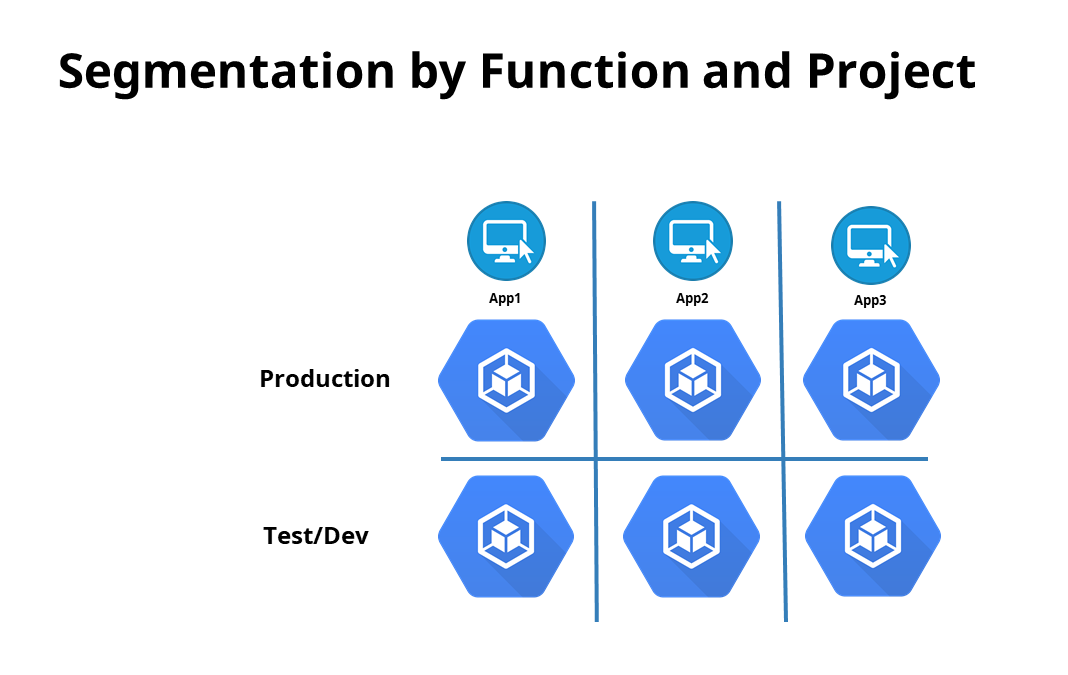
\includegraphics[width=\linewidth]{images/separation}
\label{fig:clusterSeparation}
\end{figure}

Segmentation of applications could be performed along the lines of function (Production, Development/Test), or between applications, or both. In single-cluster environments, separation could be achieved through networking or otherwise through the introduction of multiple clusters. 

A key consideration when implementing separation is the so-called "Blast Radius", a term borrowed from the military, which depicts the amount of damage an explosive would cause. In IT, it is used to assess the damage a breach, data loss, or failure of a given IT system would cause to the whole operation, in technical and financial terms.

Defining application and data security classes is part of the preparation process when introducing containers to production, and would exceed the scope of this paper.

Kubernetes itself, at the time of writing, does not provide for hard tenancy. To fully separate applications on all layers (compute, network, and storage), the use of multiple clusters is a good option. Many enterprises might thus end up with more than one Kubernetes cluster, sometimes with many more, which will, in turn, have a great effect on operations.

Also, as we're observing a trend in Enterprise IT to move from traditional perimeter-based network security to more modern zero- or low-trust networks with identity-based security and ephemeral infrastructure, having multiple, short-lived Kubernetes cluster is a likely scenario going forward.

\subsection{The principle of least privilege}

The second crucial component of security is user authentication and authorization; especially with the shift to identity-based security, Enterprise IT needs to establish a trusted identity provider and link it to its container platform.

Many Enterprise IT already have some form of central user authentication, through Microsoft Active Directory or any other Single-Sign-On provider. Kubernetes has built-in Role-Based Access Control and can restrict access to its resources based on the roles bound to a specific user or object.

Defining Roles and Responsibilities is part of the Role Engineering process during the introduction of containers, and would exceed the scope of this paper. It is, however, important in RBAC to fully embrace the principle of least privilege - only ever grant the minimum access rights required to fulfill the job, without jeopardizing efficiency though. 

A comprehensive reference for RBAC can be found in David F. Ferraiolo's book of the same name, Role-Based Access Control\cite{rbac}.

\subsection{Organizational considerations}

The third crucial component of security is departmental organization - NIST recommends that an organization changes its operational culture and technical processes to fully embrace and support agile application development.

Agile software development requires an agile organizational structure and self-organized teams to support the agile mantra “You build it, you run it” (Werner Vogels).\footnote{\textit{Orban, S. (2015)}: Enterprise DevOps: Why You Should Run What You Build. \cite{devOps}}

Without such changes, from experience, the likelihood of failing the transformation to container-based, cloud-native application development is quite high.

\subsection{Day Two operations with multiple Kubernetai}

Once all preparations have been completed, the organizational structure is about to change and multiple clusters are installed, there are a lot of configuration items and actions that need to be synchronized across all clusters.

Central user authentication and authorization is key. Authentication can be performed through an identity provider, but roles and responsibilities need to be defined for each cluster, and users need to be assigned the roles for authorization. There's only one hierarchy level on Kubernetes, roles can be bound to user objects and become effective in one or more namespaces.

Kubernetes provides two types of security policies, one for pod security and one for network security. Pod security policies, as the name implies, govern security-relevant aspects of pod specification,\footnote{See \textit{The Linux Foundation (2019)}: Pod Security Policies. \cite{podSecurity}} whereas network policies govern the allowed communication in between groups of pods and the outside world.\footnote{See \textit{The Linux Foundation (2019)}: Network Policies. \cite{netSecurity}}

As time goes on, supporting applications will need to be updated and Kubernetes itself might need to be updated unless Kubernetes is managed by a public cloud provider.

To effectively control a Kubernetes cluster and aid in troubleshooting, logging and monitoring should to be configured and enabled.

The configuration and metadata information of all deployments in a given Kubernetes cluster is stored in a distributed etcd database. This information state needs to be regularly backed up, and in case of issues, be restored.

To provide for data persistence, volumes and shared file systems need to be created for various Kubernetes clusters.

For software development and automatic deployment, it makes sense to connect the development pipeline(s) to the respective clusters, have a central image registry and establish central governance for deployment workflows.

For micro-service observability, distributed tracing and network control, a service mesh could be installed - a quite popular choice would be Istio.\footnote{See \textit{Istio Authors (2019)}: Istio - Connect, secure, control, and observe services. \cite{istio}}

All of these tasks can, of course, be performed against individual clusters with native Kubernetes tools, but once there are a couple of clusters to manage, this will get tedious and quite difficult to synchronize.

It will even get more difficult, once IaC enters the picture and Kubernetes clusters are starting to become ephemeral with the run-time environment recreated fresh with each new application deployment, fully relying on automation to implement governance and policies.

\subsection{Possible solutions}

To address all these issues, CNCF is working on Kubernetes federation and multi-cluster controlling, but the development still in its infancy and not production-ready yet.\footnote{See \textit{sig-multicluster (2019)}: Kubernetes Cluster Federation. \cite{kubeFed}}

The three big cloud providers also provide solutions to manage multiple clusters: Google Cloud has Anthos,\footnote{See \textit{Google (2019)}: Anthos - Bringing the cloud to you. \cite{googleAnthos}} Microsoft Azure has Azure Arc in Preview,\footnote{See \textit{Microsoft (2019)}: Bring Azure services and management to any infrastructure. \cite{azureArc}} and AWS is working on AWS Outposts.\footnote{See \textit{AWS (2019)}: AWS Outposts. \cite{awsOutposts}}

A popular open-source solution for this problem is Rancher, by Rancher Labs. In the next chapter, we'll have a look at whether Rancher could provide a solution to Kubernetes multi-cluster management and how it would address the issues outlined above.
